\subsection{Time Results}
\label{Time Results}
This chapter compares the efficiency of the two algorithms in terms of their time. The amount of taken by the two algorithms are graphically 
represented, analysed and a conclusion of as to which of the two algorithm is more efficient in terms of taken is reached based on figure \ref{fig:time_comparison}.
\begin{figure}[H]
  \begin{center}
      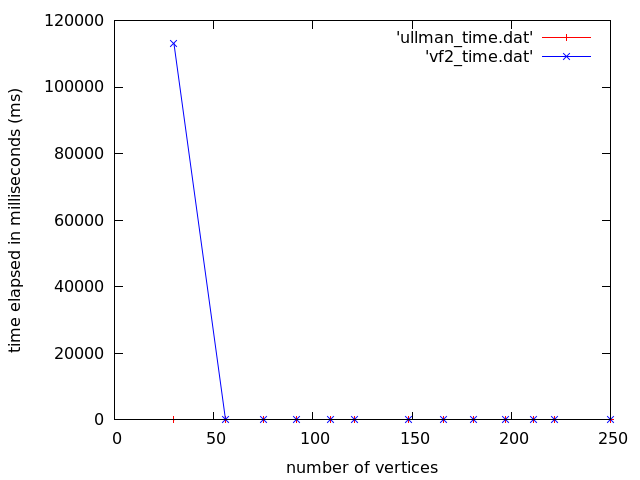
\includegraphics[width=0.8\textwidth]{time_comparison.png}
  \end{center}    
  \caption{Graph depiting the results for the time comparison between the algorithms}
  \label{fig:time_comparison}
\end{figure}

\subsubsection{Analysis of results}
Figure \ref{fig:time_comparison} depicts the comparison of the Ullman and the VF2 algorithms on the criteria of the time taken during the execution of the graph matching processes
of the respective algorithms.\newline\newline
The amount of time taken by the Ullman algorithm is depicted by the \textit{blue} line in figure \ref{fig:time_comparison}, and the time taken by VF2 algorithm 
is depicted by VF2 algorithm is depicted by the \textit{red} line in figure \ref{fig:time_comparison}.\newline\newline
Figure \ref{fig:time_comparison} depicts that the amount of time taken by the Ullman algorithm to successfully complete its graph matching processes is very 
small and consistant for the data set used in the experimentation.\newline\newline
The time taken by the VF2 algorithm however is very high for small sets of vertices, approximately \textit{40 - 60} vertices. But as the number of vertices 
increase, the amount of time declines rapidly and it equal to that of the Ullman algorithm.

\subsubsection{Conclusion}
Based of figure \ref{fig:time_comparison}, it can be deduced that the time efficiency of the Ullman and VF2 algorithms are approximately equal to each other overall,
with the exception that for small graphs, the Ullman algorithm is more efficient than the VF2 algorithm in terms of the time taken to complete the graph matching
procedures.